\chapter{Statistical Mechanics Problems}
\begin{enumerate}
	\item A system of $\mathrm{N}$ particles has only two allowed state $\mathrm{A}$ and $\mathrm{B}$. The probability for $\mathrm{A}$ is $\mathrm{P}$ and for $\mathrm{B}$ is 1-P? What is the probability for the system to be in macrostate defined by the distribution of $(r, N-r) ?$
	\begin{answer}
		 \begin{align*}
		 	\text{The probability of finding }&\mathrm{r}\text{ particle in state } \mathrm{A}=\mathrm{P}^{r}\\
		 	\text{ The probability of finding }&N-r\text{ particle in state } B=(1-P)^{N-r}\\
		 \text{	The Total no. of-ways in which}&\text{ r particle can be choosen from }N \text{- particle is }{ }^{N} C_{r}=N ! / r !(N-r) !\\
		 \text{ The probability in which r particle }&\text{are in state $A$ and $N-r$ particle in state $B$ is }=\frac{N !}{r !(N-r) !} P^{r}(1-P)^{N-r}
		 \end{align*}
	\end{answer}
	\item A one dimensiional random walker takes step to left or right with equal probability. The probability that the random walker starting from orign is back to orign after $N$ even number of step,is 
	 \begin{tasks}(2)
		\task[\textbf{a.}]$\frac{N !}{\left(\frac{N}{2}\right) !\left(\frac{N}{2}\right) !}\left(\frac{1}{2}\right)^{N}$
		\task[\textbf{b.}]$\frac{N!}{(\frac{N}{2})!(\frac{N}{2})!}$
		\task[\textbf{c.}]$2N!(\frac{1}{2})^{2N}$
		\task[\textbf{d.}] $N!(\frac{1}{2})^{N}$
	\end{tasks}
	\begin{answer}
		\begin{align*}
		\text{Probability} \quad P&=\frac{N!}{r~(N-r)}P(1-P)^{N-r}\\
		&=\frac{N !}{\left(\frac{N}{2}\right) !\left(\frac{N}{2}\right) !}\left(\frac{1}{2}\right)^{\frac{N}{2}}\left(1-\frac{1}{2}\right)^{N-\frac{N}{2}}=\frac{N!}{(\frac{N}{2})!(\frac{N}{2})!}\left( \frac{1}{2}\right) ^N
		\end{align*}
		Option \textbf{(a)} is correct
	\end{answer}
	\item Calculate the no. of microstates for a configuration of a system of $N$ distinguishable particles in which there are $n_1$ particles in a particle state $1 \& n_2$ particle in state $2,n_3$ particle .....$n_1$ particle in the $i$ th state.
	\begin{answer}
		\begin{align*}
		\text{Total No. of particle }&=N\\
		\text{No: of microstate for state}-1&={{N_C}_{n1}}\\
	\text{	No. of microstate for state }-2&=\mathrm{N}-\mathrm{n}_{1}{ }_{\mathrm{C}_{\mathrm{n}} 2}\\
\text{	No. of microstate for state }i^{\text {th }}&=N-n_{1}-n_{2} \ldots . n_{i}-1_{c_{n_{i}}}
\intertext{So\quad total number of microstate is}
\mathrm{N}_{\mathrm{C}_{\mathrm{n}_{1}}} \times \mathrm{N}-\mathrm{n}_{1} \mathrm{C}_{\mathrm{n}_{2}} &\times \mathrm{N}-\mathrm{n}_{1}-\mathrm{n}_{2} \mathrm{C}_{\mathrm{n}_{3}} \times \ldots \ldots \ldots \mathrm{N}-\mathrm{n}_{1}-\mathrm{n}_{2}-\mathrm{n}_{3}-\mathrm{ni}-1_{\mathrm{n}_{\mathrm{i}}}\\
=\frac{N !}{n_{1} !\left(N-n_{1}\right) !} &\times \frac{(N-n) !}{n_{2} !\left(N-n_{1}-n_{2}\right) !} \times \ldots \ldots \cdot \frac{\left(N-n_{1}-n_{2} \ldots n_{i}\right) !}{n_{i} !\left(N-n_{1}-n_{2} \ldots n_{i}\right) !}\\
=\frac{N !}{n_{i} !\left(N-n_{1}-n_{2} \ldots . n_{i}\right) !}&
-\text{ For distinguishable particle}\\
=\frac{1}{n_{i} !\left(N-n_{1}-n_{2} \ldots n_{i} !\right) !}& \rightarrow
\text{For indistinguishable particle}
		\end{align*}
	\end{answer}
	\item Four distinguishable coins are tossed a large no. of time write down the different microstate which may be observed \& the macrostate into which they would fall. Give the probability of the most probable macrostate.\\
	\begin{center}
	\begin{tabular}{|p{2.5cm}|p{2.7cm}|p{2.5cm}|p{2.7cm}|p{2.5cm}|}
		\hline Macrostate & Microstate coins having head up & Microstate coins having tail up & No.of microstate & Probability \\
		\hline $\mathrm{n}_{1}=4, \mathrm{n}_{2}=0$ & $\mathrm{a} \mathrm{b} \mathrm{c} \mathrm{d}$ & $-$ & 1 & $\frac{1}{16}$ \\
		\hline & $\mathrm{abc}$ & $\mathrm{d}$ & & \\
		$\mathrm{n}_{1}=3, \mathrm{n}_{2}=1$ & $\mathrm{bcd}$ & $\mathrm{a}$ & 4 & $\frac{4}{16}$ \\
		& $\mathrm{cda}$ & $\mathrm{b}$ & & \\
		& $\mathrm{dab}$ & $\mathrm{c}$ & & \\
		\hline
		 &$\mathrm{ab}$&$\mathrm{cd}$ & &\\
		 &$\mathrm{ac}$&$\mathrm{bd}$ & &\\
		 $n_1=2,n_2=3$&$\mathrm{ad}$&$\mathrm{bc}$ &6&$\frac{6}{16}$\\
		 &$\mathrm{bc}$&$\mathrm{ad}$ & &\\
		 &$\mathrm{bd}$&$\mathrm{ac}$ & &\\
		 &$\mathrm{cd}$&$\mathrm{ab}$ & &\\
		 \hline
		  &$\mathrm{a}$&$\mathrm{bcd}$ & &\\
		$n_1=1,n_2=3$&$\mathrm{b}$&$\mathrm{acd}$ &4 &$\frac{4}{16}$\\
		  &$\mathrm{c}$&$\mathrm{abd}$ & &\\
		 &$\mathrm{d}$&$\mathrm{abc}$ & &\\
		  \hline
		  	$n_1=0,n_2=1$&$-$&$\mathrm{abcd}$ &1 &$\frac{1}{16}$\\
		  	 \hline
	\end{tabular}
\end{center}
\begin{answer}
	\begin{align*}
	\text{Total no. of microstate }&=6\\
	\text{The probability of most probable state }&=6/16
	\end{align*}
\end{answer}
	\item An isolated system consist of two non-interacting spin $-1/2$ particles a \& b fixed in space \& kept in magnetic field B. Find out the total number of microstates allowed in the system.

	\begin{answer}
		$\left. \right. $\\
		\begin{table}[H]
	\begin{tabular}{|p{2.5cm}|p{2.5cm}|p{2.5cm}|p{2.5cm}|p{2.5cm}|}
		\hline
		Systemstate or macrostate  &Particlestate or Microstate & Magnetic moment &Energy  &No.of microstate  \\ \hline
		1& U \quad U&$2\mu_0$ & $-2\mu_0 B$& 1   \\ \hline
	 \multirow{ 2}{*}{1} & U \quad D & 0 & 0 & \multirow{ 2}{*}{2}\\ 
		 & U \quad D & 0 & 0 &  \\ \hline
		 3&D\quad D&$-2\mu_0$& $+-2\mu_0B$&1\\
		 \hline
	\end{tabular}
\end{table}
\begin{align*}
\intertext{Total no. of microstate $=4$ for $\operatorname{Spin}-\frac{1}{2}$ two particle system no. of accessible microstate corresponding to energy.}
E=0\text{ is }2&
\intertext{The no. of microstate for $\mathrm{N}$ no. of Spin S particle}
(2 S+1)^{N}&
\intertext{The probability of getting a macrostate in which there are r particle out of N Spin $1 / 2$ particle in spin up state}
\mathrm{N}_{\mathrm{C}_{\mathrm{r}}} \times \frac{1}{2^{\mathrm{N}}}
\end{align*}
	\end{answer}
\item We have equal amount of two identical ideal gases at the same temperature $T$ but at different pressure $P_1$ and $P_2$ in two containers of volume $V_1$ and $V_2$ respectively. The containers are connected. Find the change in entropy (The temperature after mixing also ramains same)
\begin{answer}
	\begin{align*}
	S&=Nk_B \ \ell n\left( \frac{V}{N}\right)+\frac{3}{2}Nk_B \left[\frac{5}{3}+\ell n \left(\frac{2\pi mk_BT}{h^2} \right) \right] \\
	\sum\limits_{i=1}^{2}Si&=N_1k_B\ \ell n\frac{V_i}{N}+\frac{3}{2}N_1k_B \left[\frac{5}{3}+\ell n \left(\frac{2\pi mk_BT}{h^2} \right) \right] \\
	&=Nk_B\ \ell n\frac{V_1}{N}+\frac{3}{2}Nk_B \left[\frac{5}{3}+\ell n \left(\frac{2\pi mk_BT}{h^2} \right) \right]+\\
		&=Nk_B\ \ell n\frac{V_2}{N}+\frac{3}{2}Nk_B \left[\frac{5}{3}+\ell n \left(\frac{2\pi mk_BT}{h^2} \right) \right]+\\
		&\left\{\begin{array}{l}P_{1} V_{1}=N k_{B} T \Rightarrow \frac{V_1}{N}=\frac{k_B T}{P_1}\\ P_{2} V_{2}=N k_{B} T \Rightarrow \frac{V_2}{N}=\frac{k_B T}{P_2} \end{array}\right.\\
		\sum\limits_{i=1}^{2}Si&=Nk_B\ \ell n\frac{k_B T}{P_1}+\frac{3}{2}Nk_B \left[\frac{5}{3}+\ell n \left(\frac{2\pi mk_BT}{h^2} \right) \right] +\\
		&=Nk_B\ \ell n\frac{k_B T}{P_2}+\frac{3}{2}Nk_B \left[\frac{5}{3}+\ell n \left(\frac{2\pi mk_BT}{h^2} \right) \right]
		\intertext{\textbf{Total entropy:}}
		S_T&=2Nk_B\ \ell n\frac{V_1+V_2}{2N}+\frac{3}{2}\times 2Nk_B \left[\frac{5}{3}+\ell n \left(\frac{2\pi mk_BT}{h^2} \right) \right]
		\intertext{Change in entropy}
		\Delta S&=S_T-\sum\limits_{i=1}^{2}Si=2Nk_B\ \ell n\frac{V_1+V_2}{2N}-Nk_B \ \ell n\frac{k_B T}{P_1}-NK \ \ell n\frac{k_B T}{P_2}
		\intertext{Let after mixing pressure $=P$ and after mixing total No of particle $=N+N=2 N$}
		\end{align*}
		\begin{align*}
		&\mathrm{P}\left(\mathrm{V}_{1}+\mathrm{V}_{2}\right)=2 \mathrm{Nk}_{\mathrm{B}} \mathrm{T}\hspace{6cm}\mathrm{P}\left(\mathrm{V}_{1}+\mathrm{V}_{2}\right)=2 \mathrm{Nk}_{\mathrm{B}} \mathrm{T}\\
		&\frac{\left(\mathrm{V}_{1}+\mathrm{V}_{2}\right)}{2 \mathrm{~N}}=\frac{\mathrm{k}_{\mathrm{B}} \mathrm{T}}{\mathrm{P}}\hspace{6.5cm}\frac{1}{\mathrm{P}}=\frac{\mathrm{V}_{1}+\mathrm{V}_{2}}{2 \mathrm{Nk}_{\mathrm{B}} \mathrm{T}}=\frac{\mathrm{V}_{1}}{2 \mathrm{Nk}_{\mathrm{B}} \mathrm{T}}+\frac{\mathrm{V}_{2}}{2 \mathrm{Nk}_{\mathrm{B}} \mathrm{T}}\\
		&\Delta \mathrm{S}=2 \mathrm{Nk}_{\mathrm{B}} \ \ell n \frac{\mathrm{k}_{\mathrm{B}} \mathrm{T}}{\mathrm{P}}-\mathrm{Nk}_{\mathrm{B}} \ell \mathrm{n} \frac{\mathrm{k}_{\mathrm{B}} \mathrm{T}}{\mathrm{P}_{1}}-\mathrm{Nk}_{\mathrm{B}}  \ \ell n \frac{\mathrm{k}_{\mathrm{B}} \mathrm{T}}{\mathrm{P}_{2}}\hspace{2cm}\frac{1}{\mathrm{P}}=\frac{1}{2}\left(\frac{1}{\mathrm{P}_{1}}+\frac{1}{\mathrm{P}_{2}}\right)\\
		&=N k_{\mathrm{B}}  \ \ell n \left(\frac{\mathrm{k}_{\mathrm{B}} \mathrm{T}}{\mathrm{P}}\right)^{2}-\mathrm{Nk}_{\mathrm{B}}  \ \ell n \frac{\mathrm{k}_{\mathrm{B}} \mathrm{T}}{\mathrm{P}_{1}}-\mathrm{Nk}_{\mathrm{B}}  \ \ell n \frac{\mathrm{k}_{\mathrm{B}} \mathrm{T}}{\mathrm{P}_{2}}\hspace{2cm}P=\frac{2 P_{1} P_{2}}{P_{1}+P_{2}}\\
		&=N k_{B}  \ \ell n \frac{\left(\frac{k_{B} T}{P}\right)^{2}}{\left(\frac{k_{B} T}{P_{1}}\right)\left(\frac{k_{B} T}{P_{2}}\right)}\\
		&=N k_{B}  \ \ell n \left[\frac{\left(k_{B} T\right)^{2}\left(P_{1}+P_{2}\right)^{2}}{\left(2 P_{1} P_{2}\right)^{2}} \times \frac{P_{1} P_{2}}{\left(k_{B} T\right)^{2}}\right]\\
		\Delta \mathrm{S}&=\mathrm{Nk}_{\mathrm{B}} \ell \mathrm{n} \frac{\left(\mathrm{P}_{1}+\mathrm{P}_{2}\right)^{2}}{4 \mathrm{P}_{1} \mathrm{P}_{2}}\\
		\Delta \mathrm{S}&=\mathrm{Nk}_{\mathrm{B}}  \ \ell n \frac{\left(\mathrm{P}_{1}+\mathrm{P}_{2}\right)^{2}}{4 \mathrm{P}_{1} \mathrm{P}_{2}}\quad\text{ Here we get }\Delta S>0\\
		\intertext{(We are considering identical particle. So it is a reversible case only when the particle density is same otherwise for identical gas also we will get $\Delta S>0$)}
	\end{align*}
\end{answer}
	\item Calculate the number of microstate for a free particle in 3-dimension that have momentum $p$.
	\begin{answer}
		\begin{align*}
		\mathrm{d} \tau&=\mathrm{dx} d y d z d p_{x} d p_{y} d p_{z}\\
	\textbf{	Allowed Phase Space Volume}=&\int \mathrm{d} \tau=\int \mathrm{dxdydz} \int \mathrm{dp}_{\mathrm{x}} \mathrm{dp}_{\mathrm{y}} \mathrm{dp}_{\mathrm{z}}\\
	&=V \int p^{2} d p \int_{0}^{\pi} \sin \theta d q \int_{0}^{2 \pi} d \phi=V \frac{4}{3} \pi p^{3}\\
\text{	No. of microstate }&=\frac{\mathrm{V}}{\mathrm{h}^{3}} \times \frac{4}{3} \pi \mathrm{p}^{3}
\intertext{Note : for 2. dimension.}
\int \mathrm{dx}&=\int \mathrm{dx} \int \mathrm{dy} \int \mathrm{dp}_{\mathrm{x}} \int \mathrm{dp}_{\mathrm{x}}\\
&=\int \mathrm{d}^{2} \mathrm{q} \cdot \mathrm{d}^{2} \mathrm{p} \quad=\mathrm{A} \cdot \pi \mathrm{p}^{2} \quad\{\text{ where }\mathrm{A}= \text{area} \}
\intertext{Since wave polarize in 2 dimension}
\int \mathrm{dr}&=2 \mathrm{~A} \pi \mathrm{p}^{2}
\intertext{If momentum lies between $p$ and $p+d p$}
\therefore\text{ No. of microstate }&=\frac{2 \mathrm{~A}}{\mathrm{~h}^{2}} 2 \pi \mathrm{pdp}=\frac{4 \mathrm{~A} \pi}{\mathrm{h}^{2}} \mathrm{pdp}
\intertext{If momentum lies between $\mathrm{p}$ and $\mathrm{p}+\mathrm{dp}$ then no. of microstate $=\frac{\mathrm{V}}{\mathrm{h}^{3}} 4 \pi \mathrm{p}^{2} \mathrm{dp}$}
\text{Density of state }&=\frac{\text { no. of state }}{\text { Volume }}\text{ or} \frac{\text { no. of state }}{\text { energy int erval }}
		\end{align*}
	\end{answer}
	\item Calculate the number of microstates accessible to the photon having frequency between $\nu$ and $\nu+d\nu$ confined to a 3 dimentional cavity of volume $V$
	 \begin{answer}
	 	\begin{align*}
	 	\intertext{No. of microstate in frequency range 0 to $\nu$}
	 	\Omega&=\frac{V}{h^{3}} \frac{4}{3} \pi(2 m E)^{3 / 2} \hspace{3cm}
	 	E=\frac{P^{2}}{2 m} \Rightarrow P=\sqrt{2 m} E\\
	 	&=\frac{\mathrm{V}}{\mathrm{h}^{3}} \frac{4}{3} \pi\left(\mathrm{P}^{2}\right)^{3 / 2}\hspace{3cm} \mathrm{P}=\frac{\mathrm{E}}{\mathrm{C}}=\frac{\mathrm{h\nu}}{\mathrm{C}}\\
	 	\Omega&=\frac{\mathrm{V}}{\mathrm{h}^{3}} \frac{4}{3} \pi \mathrm{P}^{3}=\frac{\mathrm{V}}{\mathrm{h}^{3}} \frac{4}{3} \pi\left(\frac{\mathrm{h\nu}}{\mathrm{c}}\right)^{3}=\frac{4}{3} \frac{\pi \mathrm{V\nu}^{3}}{\mathrm{c}^{3}}
	 	\intertext{No. of microstates in the frequency range $\nu$ and $v+d \nu$ is}
	 	\mathrm{d} \Omega&=\frac{4}{3}\  \frac{\pi \mathrm{V}}{\mathrm{c}^{3}} 3 \mathrm{\nu}^{2} \mathrm{~d} \mathrm{v}=\frac{4 \pi \mathrm{V}}{\mathrm{c}^{3}} \mathrm{\nu}^{2} \mathrm{~d} \mathrm{\nu}
	 	\intertext{Density of state}
	 	g(E)&=\text{ no. of states per unit energy range}\\
	 \text{	we have }\quad
	 	\Omega&=\frac{V}{h^{3}} \ \frac{4}{3} \ \pi(2 m E)^{3 / 2}\\
	 	\mathrm{d} \Omega&=\frac{\mathrm{V}}{\mathrm{h}^{3}} \ \frac{4}{3}\  \cdot \frac{3}{2} \pi(2 \mathrm{mE})^{1 / 2} 2 \mathrm{~m} \mathrm{dE}\\
	 	&=\frac{V}{h^{3}} \cdot 2 \pi(2 m)^{3 / 2} E^{1 / 2} d E\\
	 	&\left[\mathrm{E}=\frac{\mathrm{P}^{2}}{2 \mathrm{~m}} \Rightarrow 2 \mathrm{~m}\frac{P^2}{E}-\frac{E^2}{c^2 E}=\frac{E}{c^2}\right]\\
	 	&=\frac{V}{h^{3}} 2 \pi \left(\frac{E}{c^2} \right) ^{\frac{3}{2}}E^{\frac{1}{2}}dE\\
	 	&=\frac{V}{h^3}\ \frac{2\pi}{c^3}E^2dE\\
	 	g(E)&=\frac{d\Omega}{dE}=\frac{2\pi VE^2}{h^3 c^3}
	 	\end{align*}
	 \end{answer}
 \section{Canonical Ensemble}
	\item Show that the partition fuction of two independent (non-interacting)
	system $i$ and $j$ is given by 
	$$Z_{ij}=Z_i\times Z_j$$
	\begin{answer}
		\begin{align*}
		\intertext{We know that}
		P_{i}&=\frac{e^{-\beta E_{i}}}{Z_{i}}, P_{j}=\frac{e^{-\beta E_{j}}}{Z_{j}}\\
		E&=E_{i}+E_{j}, P_{i j}=\frac{e^{-\beta\left(E_{i}+E_{j}\right)}}{Z_{i j}}\\
		P_{i j}&=\frac{e^{-\beta E}}{Z_{i i}}=\frac{e^{-\beta\left(E_{i}+E_{j}\right)}}{Z_{i i}}=\frac{e^{-\beta E_{i}} \times e^{-\beta E_{j}}}{\dot{Z}_{i i}}\\
		\mathbf{P}_{\mathrm{ij}}&=\mathrm{P}_{\mathrm{i}} \times \mathrm{P}_{\mathrm{j}}\\
		\frac{e^{-\beta E_{i}} \times e^{-\beta E_{j}}}{Z_{i j}}&=\frac{e^{-\beta E_{i}}}{Z_{i}} \times \frac{e^{-\beta E_{j}}}{Z_{i}}\\
		\text{So  }\quad Z_{\mathrm{ij}}&=Z_{\mathrm{i}} \times Z_{\mathrm{j}}\\
	\text{	In general }Z_{i j k} \cdots \cdots&=Z_{i} \times Z_{j} \times Z_{k} \times \cdots \\
	\text{Total partition function }Z&=Z_{\text {Rotational motion }} \times Z_{\text {Translational motion }} \times Z_{\text {Vibrational motion }} \times \ldots \ldots \ldots \ldots \ldots
		\end{align*}
	\end{answer}
	\item A system consist of three independent particles localised in space. Each particle have two states of energy $O$ and $E$. When the system is in thermal equilibrium with a heat bath at temperature $T$. Calculate its partition function? 
 	\begin{answer}
 		Method :-1
 		\begin{align*}
 		\mathrm{Q}_{\mathrm{N}}(\mathrm{V}, \mathrm{T})&=\sum_{\mathrm{r}} \mathrm{g}_{\mathrm{r}} \mathrm{e}^{-\beta \mathrm{E}_{\mathrm{r}}}\\
 		Q_1 (V,T)=\sum e^{\beta E_r}=1+e^{\beta E}
 		\end{align*}
 	\end{answer}
	\item The partition function for two Bose particle each of which can occupy any of the enetgy level $0$ and $E$ 
	 \begin{tasks}(2)
		\task[\textbf{a.}]$1+e^{-2 E / K T}+2 e^{-E / K T}$
		\task[\textbf{b.}] $1+e^{-2 E / K T}+e^{-E / K T}$
		\task[\textbf{c.}]$2 \mathrm{e}^{-2 \mathrm{E} / \mathrm{KT}}+\mathrm{e}^{-\mathrm{E} / \mathrm{KT}}$
		\task[\textbf{d.}] $e^{-2 E / K T}+e^{-E / K T}$
	\end{tasks}
	\begin{answer}$\left. \right. $\\
		\renewcommand*{\arraystretch}{2}
		\begin{tabular}{llllll} 
			& $\mathbf{0}$ & $\mathbf{E}$ & Total energy & \multicolumn{2}{c}{ degeneracy } \\
			1 & aa & 0 & 0 & 1 & $\left(g_{1}\right)$ \\
			2 & a & a & E & 1 & $\left(g_{2}\right)$ \\
			3 & 0 & a & 2 E & 1 & $\left(g_{3}\right)$
		\end{tabular}
	\begin{align*}
	\mathrm{Q}_{\mathrm{N}}(\mathrm{V}, \mathrm{T})&=\sum_{\mathrm{r}} \mathrm{g}_{\mathrm{r}} \mathrm{e}^{-\beta \mathrm{E}_{\mathrm{r}}}=\mathrm{g}_{1} \mathrm{e}^{-\beta \mathrm{E}_{1}}+\mathrm{g}_{2} \mathrm{e}^{-\beta \mathrm{E}_{2}}+\mathrm{g}_{3} \mathrm{e}^{-\beta \mathrm{E}_{3}}\\
	&=1+\mathrm{e}^{-\beta E}+\mathrm{e}^{-2 \beta E}
	\end{align*}
	Correct answer is option \textbf{(b)}
	\end{answer}
	\item The partition function of single gas molecule is $Z\alpha$. The partition fuction of $N$ such non-interacting gas molecule is given by
	 \begin{tasks}(2)
		\task[\textbf{a.}]$\frac{(Z \alpha)^{N}}{N !}$
		\task[\textbf{b.}]$(Z \alpha)^{N}$
		\task[\textbf{c.}] $\mathrm{NZ} \alpha$
		\task[\textbf{d.}] $(Z \alpha)^{N} / N$
	\end{tasks}
	\begin{answer}
		\begin{align*}
		\text{For indistinguishable particle }&\frac{(Z \alpha)^{N}}{N !}\\
		\text{for distinguishable particle }&(Z \alpha)^{N}
		\end{align*}
	\end{answer}
	\item A system has energy level $E_0,2E_0,3E_0....$ where the excited state are triply degenerate. Four non-interacting Bosons are placed in this system. If the total energy of these Bosons is $5E_0$. The number of microstate is 
	 \begin{tasks}(2)
		\task[\textbf{a.}]2
		\task[\textbf{b.}]3
		\task[\textbf{c.}]4
		\task[\textbf{d.}]5
	\end{tasks}
	\begin{answer}
		\begin{align*}
		\text{Total energy }&=5 \mathrm{E}_{0}
		\intertext{For this 3 bosons must be in $E_0$ state and $1$ in $2E_0$ state.}
		\end{align*}
		\begin{figure}[H]
			\centering
			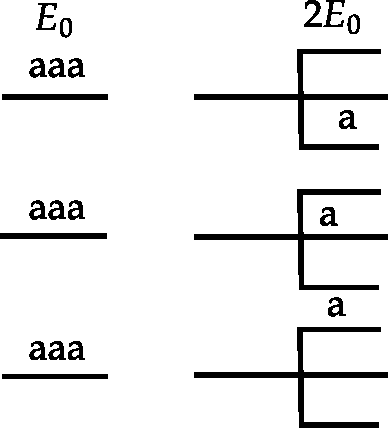
\includegraphics[height=4cm,width=4cm]{SM-problem-01}
		\end{figure}
		Correct answer is option \textbf{(b)}
	\end{answer}
	\item An ensemble of quantum harmonic oscillator is kept at a finite temperature $T$ 
	$$\mathrm{T}=\frac{1}{\mathrm{k}_{\mathrm{B}} \beta} \quad
 k_B	\text{-Boltzmann constant}$$
 The partition function of a single oscillator with energy $\left( n+1/2\right) \hbar\omega$ is given by
  \begin{tasks}(2)
 	\task[\textbf{a.}] $Z=\frac{e^{-\beta \hbar \omega / 2}}{1-e^{-\beta \hbar \omega}}$
 	\task[\textbf{b.}]$Z=\frac{e^{-\beta \hbar \omega / 2}}{1+e^{-\beta \hbar \omega}}$
 	\task[\textbf{c.}]$Z=\frac{1}{1-e^{-\beta \hbar \omega}}$
 	\task[\textbf{d.}] $Z=\frac{1}{1+e^{-\beta \hbar \omega}}$
 \end{tasks}
	
	
	
	
	
	
	
	
	
	
	
	
	
	
	
	
	
	
	
	
	
	
	
\end{enumerate}